\documentclass[handout]{beamer}
\usepackage[T1]{fontenc}
\usepackage[utf8]{inputenc}
\usepackage{lmodern}
\usepackage[english]{babel}
\usepackage{tikz}
\usetikzlibrary{patterns}
\usepackage{graphicx}
\usepackage{multicol}
\usepackage{float}
\usepackage{newfloat}


\usetheme{Berlin}
\usecolortheme{beaver}
\usefonttheme{structuresmallcapsserif}
%\setbeamertemplate{itemize item}[default]
%\setbeamertemplate{enumerate item}[default]
\setbeamercolor{item projected}{bg=darkred,fg=white}
\beamertemplateballitem

\setbeamertemplate{caption}{\raggedright\insertcaption\par}

%\setbeamercolor{section number projected}{bg=darkred,fg=white}

\makeatletter

\defbeamertemplate*{footline}{myfootline}
{
  \leavevmode%
  \hbox{%
  \begin{beamercolorbox}[wd=.333333\paperwidth,ht=2.25ex,dp=1ex,left]{title in head/foot}%
    \usebeamerfont{author in head/foot}\insertshortauthor
  \end{beamercolorbox}%
  \begin{beamercolorbox}[wd=.333333\paperwidth,ht=2.25ex,dp=1ex,center]{title in head/foot}%
    \usebeamerfont{institute in head/foot}\insertshortinstitute
  \end{beamercolorbox}%
  \begin{beamercolorbox}[wd=.333333\paperwidth,ht=2.25ex,dp=1ex,right]{title in head/foot}%
    \usebeamerfont{date in head/foot}\insertshortdate{}\hspace*{2em}
    \insertframenumber{} / \inserttotalframenumber\hspace*{2ex} 
  \end{beamercolorbox}}%
  \vskip0pt%
}
\makeatother

 \setbeamertemplate{footline}[myfootline]


\setbeamersize{text margin left=0.5cm,text margin right=0.5cm}


\title[\textsc{Fabrication and measurements of NIS junctions}]
{
\textsc{Fabrication and measurements of\\
NIS junctions to characterize\\
plasma etching}
}


\author[     Nicolas \textsc{Paillet}]
{
Nicolas \textsc{Paillet}\\
{\footnotesize Under the supervision of\\
Pr. Jukka \textsc{Pekola} \& Quentin \textsc{Rafhay}}
}

\institute[Grenoble INP Phelma]
{       
  \begin{multicols}{2}
  Grenoble INP Phelma\\
  \vspace{2mm}
  
 \includegraphics[width=12mm]{logo_phelma.png}
 
  Aalto University\\
  \vspace{2mm}
  
  \includegraphics[width=10mm]{logo_aalto.png}
  \end{multicols}
}

\date{5 October 2015}

\begin{document}
\logo{\includegraphics[width=1.5cm]{logo_phelma.png}}

    \begin{frame}
        \titlepage
    \end{frame}

    \begin{frame}
        \frametitle{\textsc{Outline}}
        \tableofcontents
    \end{frame}

    \section{Introduction}
        \begin{frame}
        \frametitle{Introduction}
    
            The PICO Group : Heat transport at low temperature, single-electron counting, redefining the ampere.
        
            Context : Evaporator nicknamed LISA and plasma etching
    
            \begin{figure}[H]
                \includegraphics[width=40mm]{LISA.JPG}
                \caption{Picture of the evaporator LISA}
            \end{figure}
        \end{frame}

    \section{Theory}
    \subsection*{Theory}
        \begin{frame}
        \frametitle{Superconductivity}
        \begin{itemize}
        
            \item Superconductivity 
            
            \item Cooper pairs
            \begin{figure}[H]
                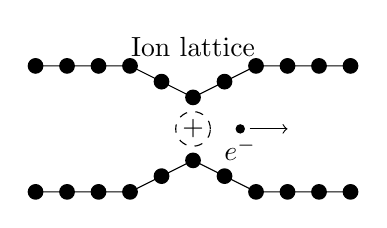
\begin{tikzpicture}[scale=0.4]
                \draw (0,0)--(3,0)--(5,1)--(7,0)--(10,0);
                \draw (0,4)--(3,4)--(5,3)--(7,4)--(10,4);
                \fill (0,0)circle(0.25);
                \fill (1,0)circle(0.25);
                \fill (2,0) circle(0.25);
                \fill (3,0) circle(0.25);
                \fill (4,0.5) circle(0.25);
                \fill (5,1) circle(0.25);
                \fill (6,0.5) circle(0.25);
                \fill (7,0) circle(0.25);
                \fill (8,0) circle(0.25);
                \fill (9,0) circle(0.25);
                \fill (10,0) circle(0.25);
                \fill (0,4) circle(0.25);
                \fill (1,4) circle(0.25);
                \fill (2,4) circle(0.25);
                \fill (3,4) circle(0.25);
                \fill (4,3.5) circle(0.25);
                \fill (5,3) circle(0.25);
                \fill (6,3.5) circle(0.25);
                \fill (7,4) circle(0.25);
                \fill (8,4) circle(0.25);
                \fill (9,4) circle(0.25);
                \fill (10,4) circle(0.25);
                \draw (5,4)node[above]{Ion lattice};
                \fill (6.5,2)circle(0.15);
                \draw [->](6.8,2)--(8,2);
                \draw (6.5,2)node[below]{$e^-$};
                \draw [dashed] (5,2)circle(0.55);
                \draw (5,2) node{$+$};
                \end{tikzpicture}
                \caption{Schematics explaining the cooper pairing}
            \end{figure}
            \end{itemize}
            \end{frame}
            \begin{frame}
            \frametitle{Density of states}
            \begin{itemize}
            \item Density of states and NIS junction
            
            
            \begin{minipage}[c]{0.45\textwidth}
            \begin{footnotesize}
                \begin{equation*}
                N(E)=\left\{ 
                \begin{array}{lr}
                \displaystyle
                N_0\dfrac{E}{\sqrt{E^2-\Delta^2}} &\text{ if } |E|>\Delta\\
                0 &\text{ if } |E|<\Delta
                \end{array}
                \right.
                \end{equation*}
                \end{footnotesize}
            \end{minipage}
            \begin{minipage}[c]{0.45\textwidth}
            \begin{figure}
                \centering
                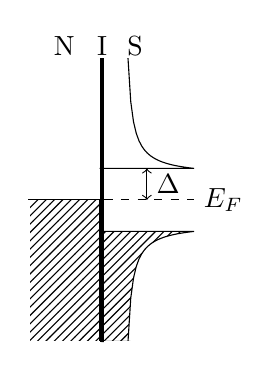
\begin{tikzpicture}[scale=0.3]
                \draw [domain=0.2:3] plot(\x,{1+1/\x})--++(-4,0);
                \draw [pattern=north east lines, pattern color=black] [domain=0.2:3] plot(\x,{-1-1/\x})--++(-3.9,0)--++(0,-4.66)--++(1.2,0);
                \draw [color=white,thick](-0.8,-6)--(1,-6);
                \fill (-1,6)--(-0.8,6)--(-0.8,-6)--(-1,-6)--cycle;
                \draw [pattern=north east lines, pattern color=black] (-4,-6) rectangle (-1,0);
                \draw [color=white,thick] (-1,-6)--(-4,-6)--(-4,0);
                \draw [<->] (1,0)--(1,1.33)node[midway,right]{$\Delta$};
                \draw (-4,0)--(-1,0);
                \draw [dashed](-0.8,0)--(3,0);
                \draw (3,0)node[right]{$E_F$};
                \draw (-2.5,6.5)node{N};
                \draw (-0.9,6.5)node{I};
                \draw (0.5,6.5)node{S};
                \end{tikzpicture}
                \caption{Density of states for a junction}
            \end{figure}
            \end{minipage}
            \item Dynes density of states : leakage current
        \end{itemize}
        \end{frame}
    \section{Experimental methods}
    \subsection*{Experimental methods}
    \begin{frame}
    \frametitle{Cleanroom Process}
    \centering{Cross section of the wafer during its preparation}
    \begin{figure}[H]
       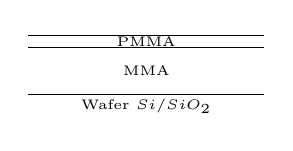
\begin{tikzpicture}[scale=0.3]
                    \draw (0,0)--(10,0);
                    \draw (5,-0.5) node{{\tiny Wafer $Si/SiO_2$}};
                    \draw (0,2)--(10,2);
                    \draw (5,1)node{{\tiny MMA}};
                    \draw (0,2.5)--(10,2.5);
                    \draw (5,2.25) node{{\tiny PMMA}};
        \end{tikzpicture}
        \begin{tikzpicture}[scale=0.3]
        \draw [->,thick](0,1)--(1,1)node[midway,above]{{\tiny EBL}};
        \draw [color=white](0,-1)--(0.1,-1);
        \end{tikzpicture}
        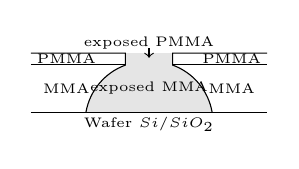
\begin{tikzpicture}[scale=0.3]
        \fill [color=gray!20](2.33,0) arc(170:110:2.6)--(4,2.5)--(6,2.5)--(6,2) arc(70:10:2.6);
                \draw (0,0)--(10,0);
                \draw (5,-0.5) node{{\tiny Wafer $Si/SiO_2$}};
                \draw (2.33,0) arc(170:110:2.6)--(4,2.5)--(0,2.5);
                \draw (7.67,0) arc(10:70:2.6)--(6,2.5)--(10,2.5);
                
                \draw (0,2)--(4,2);
                \draw (6,2)--(10,2);
                \draw (1.5,1) node{{\tiny MMA}};
                \draw (8.5,1) node{{\tiny MMA}};
                \draw (1.5,2.25) node{{\tiny PMMA}};
                \draw (8.5,2.25) node{{\tiny PMMA}};
                \draw (5,2.25)node[above]{{\tiny exposed PMMA}};
                \draw [->](5,2.7)--(5,2.3);
                 \draw (0,0)--(10,0);
                \draw (5,1)node{{\tiny exposed MMA}};
                \end{tikzpicture}
                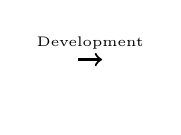
\begin{tikzpicture}[scale=0.3]
                \draw [->,thick](0,1)--(1,1)node[midway, above]{{\tiny Development}};
                \draw [color=white](0,-1)--(0.1,-1);
                \end{tikzpicture}
                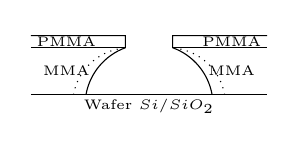
\begin{tikzpicture}[scale=0.3]
                \draw (0,0)--(10,0);
                \draw (5,-0.5) node{{\tiny Wafer $Si/SiO_2$}};
                \draw (2.33,0) arc(170:110:2.6)--(4,2.5)--(0,2.5);
                \draw (7.67,0) arc(10:70:2.6)--(6,2.5)--(10,2.5);
                \draw [dotted](1.8,0) arc(170:98:2.4);
                \draw [dotted] (8.2,0) arc(10:82:2.4);
                \draw (0,2)--(4,2);
                \draw (6,2)--(10,2);
                \draw (1.5,1) node{{\tiny MMA}};
                \draw (8.5,1) node{\tiny {MMA}};
                \draw (1.5,2.25) node{{\tiny PMMA}};
                \draw (8.5,2.25) node{{\tiny PMMA}};
                \end{tikzpicture}
                \end{figure}
                
                \centering{Cross-section during of an evaporation}
    \begin{figure}
        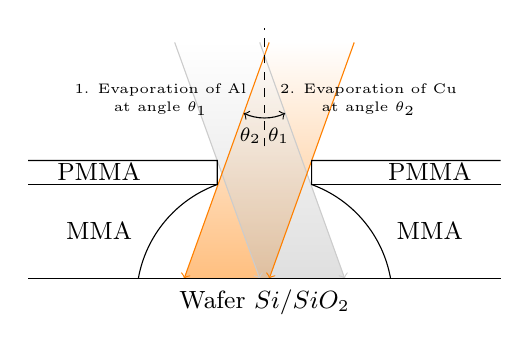
\begin{tikzpicture}[scale=0.6]
               \shadedraw[bottom color=orange,top color=white, draw=orange, fill opacity=0.5,draw opacity=0](5.1,5)--(3.3,0)--(5.1,0)--(6.9,5)-- cycle;
                \shadedraw[bottom color=gray!50,top color=white, draw=gray!40, fill opacity=0.5, draw opacity=0](4.9,5)--(6.7,0)--(4.9,0)--(3.1,5)--cycle;   
                \draw [color=gray!40,->] (4.9,5)--(6.7,0);
                \draw [color=gray!40,->] (3.1,5)--(4.9,0);  
                \draw [color=orange,->] (5.1,5)--(3.3,0);
                \draw [color=orange,<-] (5.1,0)--(6.9,5);
                          
                \draw (0,0)--(10,0);
                \draw (5,-0.5) node{{\small Wafer $Si/SiO_2$}};
                \draw (2.33,0) arc(170:110:2.6)--(4,2.5)--(0,2.5);
                \draw (7.67,0) arc(10:70:2.6)--(6,2.5)--(10,2.5);
                \draw (0,2)--(4,2);
                \draw (6,2)--(10,2);
                \draw (1.5,1) node{{\small MMA}};
                \draw (8.5,1) node{{\small MMA}};
                \draw (1.5,2.25) node{{\small PMMA}};
                \draw (8.5,2.25) node{{\small PMMA}};
                \draw [dashed](5,2.8)--(5,5.3);
                \draw [->] (5,3.4) arc(-90:-116:1);
                \draw (2.8,4) node{{\tiny 1. Evaporation of Al}};
                \draw(2.8,3.6) node{\tiny {at angle $\theta_1$}} ;               
                \draw (4.7,3.4)node[below]{{\scriptsize $\theta_2$}};
                \draw [->] (5,3.4) arc(-90:-64:1);
                \draw (7.2,4)node {{\tiny 2. Evaporation of Cu}};
                \draw (7.2,3.6)node{{\tiny at angle $\theta_2$}};
                \draw (5.3,3.4)node[below]{{\scriptsize $\theta_1$}};
            \end{tikzpicture} 
    \end{figure}
       
    \end{frame}
    \begin{frame}
        \frametitle{Cleanroom Process}
        \begin{itemize}
        \item O$_2$ valve : Oxidation
        \item Plasma Gun (with Ar valve) : \begin{itemize}
            \item Low power : Resist weakening $\rightarrow$ Easier Lift-off
            \item High Power : Plasma Etching $\rightarrow$ Etch materials
        \end{itemize}
        \end{itemize}
        
        \begin{multicols}{3}
             \begin{center}            
            \includegraphics[width=40mm]{SEMexemple.jpg}\\
            {\scriptsize Normal mode} 
            \end{center}
            
            \begin{center}
            \includegraphics[width=40mm]{SEMexemplese2.jpg}\\
             {\scriptsize Secondary electron mode}
             \end{center}
                          
            \begin{center}
            \includegraphics[width=40mm]{SEMexemplefail.jpg}\\
            {\scriptsize Failed sample}
            \end{center}
        \end{multicols}
        \centering{SEM images of some samples}
        
    \end{frame}
    
    \begin{frame}
        \frametitle{Dilution cryostat}
        \centering        
        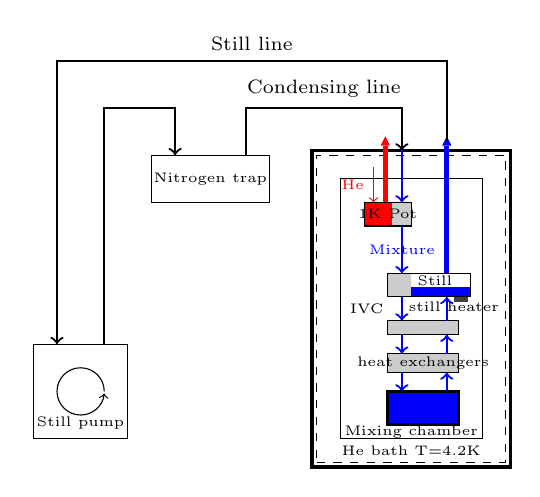
\begin{tikzpicture}[scale=0.6]

\draw (0,2)--(0,4)--(2,4)--(2,2)--cycle;
\draw [->](1.5,3) arc(0:355:0.5);
\draw (1,2)node[above]{\tiny Still pump};

\draw [thick,->](1.5,4)--(1.5,9)--(3,9)--(3,8);
\draw (2.5,8)--(5,8)--(5,7)--(2.5,7)--cycle;
\draw (3.75,7.5)node{{\tiny Nitrogen trap}};
\draw [thick,->] (4.5,8)--(4.5,9)--(7.8,9)node[midway,above]{{\scriptsize Condensing line}}--(7.8,8.1);

\draw [very thick] (5.9,1.4)--(10.1,1.4)--(10.1,8.1)--(5.9,8.1)--cycle;%HEdewar
\draw (8,1.75)node{{\tiny He bath T=4.2K}};
\draw [dashed] (6,1.5)--(10,1.5)--(10,8)--(6,8)--cycle;
\draw (6.5,2)--(9.5,2)--(9.5,7.5)--(6.5,7.5)--cycle;%IVC
\draw (6.5,4.75)node[right]{{\tiny IVC}};
\fill [color=red] (7,7)--(7.6,7)--(7.6,6.5)--(7,6.5)--cycle;

\draw [color=red,->](7.2,7.75)--(7.2,7)node[midway, left]{{\tiny He}};
\fill [color=red] (7.4,7)--(7.5,7)--(7.5,8.2)--(7.4,8.2)--cycle;%He
\fill [color=red] (7.35,8.2)--(7.55,8.2)--(7.45,8.4)--cycle;%He
\fill [color=gray!40] (7.6,7)--(7.6,6.5)--(8,6.5)--(8,7)--cycle;%heat exc
\draw (7,7)--(8,7)--(8,6.5)--(7,6.5)--cycle;%1Kpot
\draw (7.5,6.75)node{{\tiny 1K Pot}};

\draw [color=blue,->, thick](7.8,8.1)--(7.8,7);%mixt
\fill [color=gray!40] (7.5,5.5)--(7.5,5)--(8,5)--(8,5.5)--cycle;
\fill [color=blue] (8,5)--(8,5.2)--(9.25,5.2)--(9.25,5)--cycle;
\draw (7.5,5.5)--(7.5,5)--(9.25,5)--(9.25,5.5)--cycle;%still
\fill [color=gray!150] (8.9,5)--(9.2,5)--(9.2,4.9)--(8.9,4.9)--cycle;
\draw (8.9,4.8)node{{\tiny still heater}};
\draw [color=blue,->,thick] (7.8,5)--(7.8,4.5); 
\fill [color=gray!40] (7.5,4.5)--(7.5,4.2)--(9,4.2)--(9,4.5)--cycle;

\draw (7.5,4.5)--(7.5,4.2)--(9,4.2)--(9,4.5)--cycle;
\draw [color=blue,->,thick](7.8,4.2)--(7.8,3.8);
\draw (8.5,5.35)node{{\tiny Still}};
\draw [color=blue,->,thick](7.8,6.5)--(7.8,5.5)node[midway]{{\tiny Mixture}};%mixt
\fill [color=gray!40] (7.5,3.8)--(7.5,3.4)--(9,3.4)--(9,3.8)--cycle;
\draw (7.5,3.8)--(7.5,3.4)--(9,3.4)--(9,3.8)--cycle;
\draw (8.25,3.6)node{{\tiny heat exchangers}};
\draw [color=blue,->, thick](7.8,3.4)--(7.8,3);
\fill [color=blue] (7.5,3)--(7.5,2.3)--(9,2.3)--(9,3)--cycle;
\draw [very thick] (7.5,3)--(7.5,2.3)--(9,2.3)--(9,3)--cycle;
\draw (8,2.15)node{{\tiny Mixing chamber}};
\draw [color=blue,->, thick] (8.75,3)--(8.75,3.4);

\draw [color=blue,->,thick] (8.75,4.5)--(8.75,5);
\draw [color=blue,->,thick] (8.75,3.8)--(8.75,4.2);
\fill [color=blue] (8.7,5.5)--(8.8,5.5)--(8.8,8.2)--(8.7,8.2)--cycle;
\fill [color=blue] (8.65,8.2)--(8.85,8.2)--(8.75,8.4)--cycle;
\draw [->,thick] (8.75,8.3)--(8.75,10)--(0.5,10)node[midway,above]{{\scriptsize Still line}}--(0.5,4);

\end{tikzpicture}

        \centering{Schematics representing the functioning of a dilution cryostat. In red $^4$He, in blue $^3$He/$^4$He mixture and in grey, heat exchangers.}
    \end{frame}
    
    
    \section{Experimental Protocol}
    \subsection*{Experimental Protocol}
    \begin{frame}
        \frametitle{\textsc{Settings}}
    
    \begin{multicols}{2}
        
    
        \begin{itemize}
            \item{\small 4 Pads pattern}
         \end{itemize}   
     
     \begin{center}
        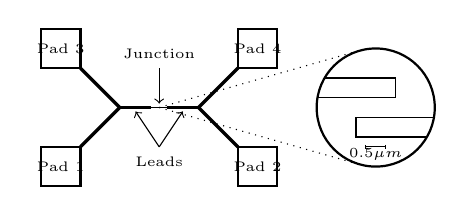
\begin{tikzpicture}[scale=0.5]
                    \draw [thick](0,0)--++(1,0)--++(0,1)--++(-1,0)--cycle;
                    \draw [thick](0,3)--++(1,0)--++(0,1)--++(-1,0)--cycle;
                    \draw [thick](5,0)--++(1,0)--++(0,1)--++(-1,0)--cycle;
                    \draw [thick](5,3)--++(1,0)--++(0,1)--++(-1,0)--cycle;
                    \draw [very thick](1,1)--(2,2);
                    \draw [very thick](1,3)--(2,2);
                    \draw [very thick](5,1)--(4,2);
                    \draw [very thick](5,3)--(4,2);
                    \draw [very thick](2,2)--(2.8,2);
                    \draw [very thick](4,2)--(3.2,2);
                    \draw (2.8,2)--(3.2,2);
                    \draw [->] (3,3)--(3,2.1);
                    \draw (3,3)node[above]{\tiny{Junction}};
                    \draw (0.5,0.5)node{\tiny{Pad 1}};
                    \draw (0.5,3.5) node{\tiny{Pad 3}};
                    \draw (5.5,0.5)node{\tiny{Pad 2}};
                    \draw (5.5,3.5)node{\tiny{Pad 4}};
                    \draw [->] (3,1)--(2.4,1.9);
                    \draw [->] (3,1)--(3.6,1.9);
                    \draw (3,1)node[below]{\tiny{Leads}};
                    \draw [dotted,thin] (3,2)--(8.1,3.45);
                    \draw [dotted,thin] (3,2)--(8.1,0.55);
                    \draw [thick](8.5,2) circle(1.5);
                    \draw (7.2,2.75)--(9,2.75)--(9,2.25)--(7.02,2.25);
                    \draw (9.8,1.25)--(8,1.25)--(8,1.75)--(9.98,1.75);
                    \draw (8.25,1.05)--(8.25,0.95);
                    \draw (8.75,1.05)--(8.75,0.95);
                    \draw (8.25,1)--(8.75,1);
                    \draw (8.5,0.8)node{\tiny{0.5$\mu m$}};
            \end{tikzpicture}
           Drawings of the pattern used
           \end{center}
            \end{multicols}
            
            \begin{itemize}
            \begin{small}
                \item{4x5 matrix with 4 Surface areas : 0.5 to 2 by 0.5$\mu m^2$ and 5 EBL dose from 2000 to 3000 by 250 $c/\mu m^2$}
                \item{Development 20s MIBK, 20s Methyglycol, IPA}
                \item{Evaporation : Al 20nm, Cu 25nm}
                \item{Optionnal : Strong Oxidation (10min, 200mbar), and/or Plasma Etching, and/or Tunnel barrier Oxidation (2min, 2mbar)}
                \item{4 probe measurements with a probestation}
                \item{Eventually : Low temperature measurements : I-V}
                \end{small}
            \end{itemize}  
                
    \end{frame}

    \section{Results}
        \subsection{Room temperature results}
    \begin{frame}
        \frametitle{Reference samples (Without Plasma Etching)}
        \begin{multicols}{2} 
            \includegraphics[width=60mm]{Rclean.png}\\
            \begin{small}
            \hfill Strong Oxidation (10min/200mbar)
            \vspace{1mm}
            
            \hfill $RS=7198 \Omega.\mu m^2$
            \end{small}
            \includegraphics[width=60mm]{ConductanceFitOx.png}

            \begin{small}
            
            
            Clean Contact Al + Cu\\
            \vspace{2mm}
            
            $R=\sum_{Cu,Al}\dfrac{\rho l}{S}\simeq 78 \Omega$\\
            \end{small}
            \vspace{4mm}
            
            \includegraphics[width=60mm]{ConductanceFitStrongOx.png}\\
            \vspace{3mm}
            
            \begin{small}
            Tunnel junction (2min/2mbar)\\
            \vspace{2mm}
            
            $RS=763 \Omega.\mu m^2$
            \end{small}
                
        \end{multicols}
                
    \end{frame}
    
    \begin{frame}
        \frametitle{Position of the sample}
        \begin{itemize}
            \item Samples with Strong Oxidation, Plasma etching 10 min, Clean contact, before the Oxygen Cleaning. 
        \end{itemize}

        \centering\includegraphics[width=90mm]{R_Position.png}\\
        $\Rightarrow$ {\small Plasma is homogeneous \& 10min seem enough to etch the Oxide\\No surface dependance, same order of magnitude as clean contact.}
    \end{frame}
     
     \begin{frame}
        \frametitle{Duration of the Plasma Etching}
        \begin{itemize}
            \item Samples with Strong Oxidation, Plasma etching, Clean contact.
            \end{itemize}
        \begin{multicols}{2}
        \begin{itemize}
            \item Before the Oxygen Cleaning 
            \end{itemize}
            \includegraphics[width=174pt]{R_TimeBefore.png}
            
            
            \begin{itemize}
            \item After the Oxygen Cleaning
            \end{itemize}
            \includegraphics[width=174pt]{R_TimeAfter.png}
            
        \end{multicols}
                
        $\Longrightarrow$ Similar results for totally different parameters before and after the cleaning. Before $\longrightarrow$ 10 min of Plasma was a good time. After the cleaning $\longrightarrow$ less than 5 min is enough \& 10 min is too much.
        
        \end{frame}
        
        \begin{frame}
            \frametitle{Plasma Problems}          
        \begin{itemize}
            \item Samples with Strong Oxidation, Plasma Etching 10 min , Tunnel barrier.
        \end{itemize}

        \begin{multicols}{2}
            \begin{itemize}
                \item Before Oxygen Cleaning
            \end{itemize}
            \centering\includegraphics[width=45mm]{Burned2.png}
            
            \begin{itemize}
                \item After Oxygen Cleaning
            \end{itemize}
            \centering\includegraphics[width=45mm]{Burned1.png}
        \end{multicols}        
        
        $\Longrightarrow$ Exact same parameters, before the cleaning : resist burned,\\after the cleaning : unidentified areas.
    \end{frame}
    
    \begin{frame}
        \frametitle{Wafer Etching}
        \begin{itemize}
            \item Sample with Strong Oxidation, Plasma Etching 10 min, Tunnel barrier, after Oxygen Cleaning.
        \end{itemize}
        \begin{multicols}{2}
             \centering\includegraphics[width=160pt]{tilt3.png}
             
             \centering\includegraphics[width=160pt]{tilt4.png}
        \end{multicols}
       SEM images with a tilted angle : The darkest area is a hole in the wafer.
            
    \end{frame}
    
    \subsection{Low Temperature Measurements}
    \begin{frame}
        \frametitle{Tunnel barrier before Oxygen Cleaning}
        
        \begin{itemize}
            \item Sample with Tunnel barrier (NIS) without Plasma
            \end{itemize}
            
            \centering\includegraphics[width=90mm]{BeforeLISAOx.png}\\
            \centering{Current in function of bias voltage applied}
        \begin{itemize}    
        \item Leakage $\simeq$ $10^{-4}$ $\rightarrow$ Correct junction
        \end{itemize}
        
    \end{frame}
    
%     \begin{frame}
%         \frametitle{Tunnel barrier after Oxygen Cleaning}
%         
%         \begin{itemize}
%             \item Sample with Tunnel barrier (NIS), without Plasma, after the Oxygen Cleaning
%             \end{itemize}
%             \includegraphics[width=90mm]{AfterLISAOx.png}\\
%             Current in function of bias voltage
%             
%         Leakage $\simeq$ $10^{-4}$ $\rightarrow$ Correct Leakage
%         \end{frame}
        
        \begin{frame}
        \frametitle{Tunnel barrier with Plasma Etching}
        \begin{itemize}
            \item Sample with Strong Oxidation, Plasma Etching 2min30s, Tunnel barrier, after the Oxygen Cleaning.
        \end{itemize}
        
        \centering\includegraphics[width=80mm]{PlasmaOx.png}\\
        \centering Current in function of bias voltage
        
        \begin{itemize}
            \item Leakage $\simeq$ $10^{-2}$ The leakage is quite bad but...
        \end{itemize}   
    
    \end{frame}
    
    \begin{frame}
    \frametitle{Tunnel barrier reference for previous sample}
        \begin{itemize}
            \item Sample with Tunnel barrier, after the Oxygen cleaning.
        \end{itemize}
        \centering\includegraphics[width=85mm]{RegularOxRef.png}\\
        \centering Current in function of bias voltage
        
        \begin{itemize}
            \item Leakage $\simeq$ $10^{-2}$ $\rightarrow$ Same order of magnitude for plasma etched sample and reference : something else wrong with the LISA
        \end{itemize}

    \end{frame}
    \section{Conclusion}
    \subsection*{Conclusion}
    \begin{frame}
           \frametitle{Summary}
          \begin{itemize}
               \item Studied bibliography to understand important points of theory
               \item Learned and getting used to use cleanroom tools
               \item Set up an experimental protocol
               \item Learned to cool down and warm up a dilution cryostat
               \item Made measurements at room and low temperature
               \item Exploited and interpreted the results 
           \end{itemize}
           
    \end{frame}
    \begin{frame}
        \begin{LARGE}
        
        \centering    
        \textbf{Thank you for your attention !}
        \vspace{0.5cm}
        
        \textbf{If you have any questions please ask.}
        
        \end{LARGE}

       \end{frame}
       
      
    \end{document}
